\documentclass[class=article,border=1pt]{standalone}
\usepackage[dvipsnames]{xcolor}
\usepackage{tikz}
\usetikzlibrary{arrows.meta}
\begin{document}
\pagestyle{empty}
\thispagestyle{empty}
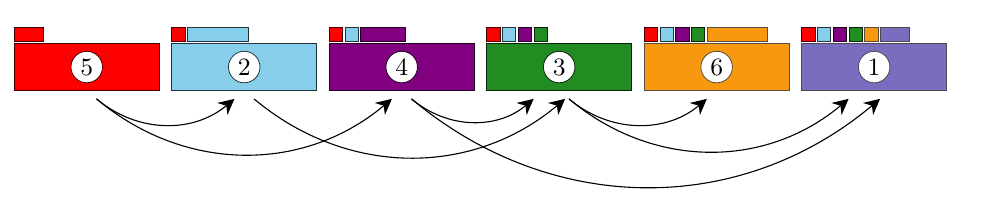
\begin{tikzpicture}
%
\def\colours{{"Red", "SkyBlue", "Purple", "ForestGreen", "YellowOrange", "Periwinkle"}}
\path[use as bounding box] (-0.75,0.5) rectangle (11,-1.5);
%
\newcommand{\vertex}[4]{
  \pgfmathparse{\colours[#3]}
  \edef\mycolour{\pgfmathresult}

  \draw[fill={\mycolour},draw=\mycolour!25!black,line width=0.1mm] (#1-0.92, 0.3) rectangle (#1+0.92, -0.3);
  \draw[fill=white,draw=\mycolour!25!black,line width=0.1mm] (#1, 0) circle (0.2);

  \foreach \n in {0,...,#3}{
    \pgfmathparse{\colours[\n]};
    \edef\barcolour{\pgfmathresult}
    \draw[fill=\barcolour,draw=black!75!\barcolour,line width=0.1mm] (#1-0.92+\n/5, 0.3+0.03) rectangle (#1-0.92+\n/5+1/5-0.03, 0.5);
  };
  \foreach \n in {#3,...,#3}{
    \pgfmathparse{\colours[\n]};
    \edef\barcolour{\pgfmathresult}
    \draw[fill=\barcolour,draw=black!75!\barcolour,line width=0.1mm] (#1-0.92+\n/5, 0.3+0.03) rectangle (#1-0.92+\n/5+#2/5-0.03, 0.5);
  }

  \node[anchor=center] at (#1, 0) {\small #4};
  \node[anchor=center] (#4) at (#1, -0.3) {};
  \node[anchor=center] (#4pre) at (#1-0.2, -0.3) {};
  \node[anchor=center] (#4aft) at (#1+0.2, -0.3) {};
}
%
\vertex{0}{2}{0}{5}
\vertex{2}{4}{1}{2}
\vertex{4}{3}{2}{4}
\vertex{6}{1}{3}{3}
\vertex{8}{4}{4}{6}
\vertex{10}{2}{5}{1}
%
\begin{scope}[-{Stealth[length=2mm, width=2mm]}]
  \draw [bend right=40] (5) edge (4);
  \draw [bend right=40] (5) edge (2);
  \draw [bend right=40] (2) edge (3aft);
  \draw [bend right=40] (4) edge (3pre);
  \draw [bend right=40] (3) edge (6);
  \draw [bend right=40] (4) edge (1aft);
  \draw [bend right=40] (3) edge (1pre);
\end{scope}
%
\end{tikzpicture}
\end{document}
